\documentclass[12pt]{article}

\usepackage{tikz} % картинки в tikz
\usepackage{microtype} % свешивание пунктуации

\usepackage{array} % для столбцов фиксированной ширины

\usepackage{indentfirst} % отступ в первом параграфе

\usepackage{sectsty} % для центрирования названий частей
\allsectionsfont{\centering}

\usepackage{amsmath} % куча стандартных математических плюшек

\usepackage[top=2cm, left=1.5cm, right=1.5cm, bottom=2cm]{geometry} % размер текста на странице

\usepackage{lastpage} % чтобы узнать номер последней страницы

\usepackage{enumitem} % дополнительные плюшки для списков
%  например \begin{enumerate}[resume] позволяет продолжить нумерацию в новом списке
\usepackage{caption}


\usepackage{fancyhdr} % весёлые колонтитулы
\pagestyle{fancy}
\lhead{Теория вероятностей}
\chead{}
\rhead{2016-10-27, праздник номер раз :)}
\lfoot{}
\cfoot{}
\rfoot{\thepage/\pageref{LastPage}}
\renewcommand{\headrulewidth}{0.4pt}
\renewcommand{\footrulewidth}{0.4pt}



\usepackage{todonotes} % для вставки в документ заметок о том, что осталось сделать
% \todo{Здесь надо коэффициенты исправить}
% \missingfigure{Здесь будет Последний день Помпеи}
% \listoftodos --- печатает все поставленные \todo'шки


% более красивые таблицы
\usepackage{booktabs}
% заповеди из докупентации:
% 1. Не используйте вертикальные линни
% 2. Не используйте двойные линии
% 3. Единицы измерения - в шапку таблицы
% 4. Не сокращайте .1 вместо 0.1
% 5. Повторяющееся значение повторяйте, а не говорите "то же"



\usepackage{fontspec}
\usepackage{polyglossia}

\setmainlanguage{russian}
\setotherlanguages{english}

% download "Linux Libertine" fonts:
% http://www.linuxlibertine.org/index.php?id=91&L=1
\setmainfont{Linux Libertine O} % or Helvetica, Arial, Cambria
% why do we need \newfontfamily:
% http://tex.stackexchange.com/questions/91507/
\newfontfamily{\cyrillicfonttt}{Linux Libertine O}

\AddEnumerateCounter{\asbuk}{\russian@alph}{щ} % для списков с русскими буквами


%% эконометрические сокращения
\DeclareMathOperator{\Cov}{Cov}
\DeclareMathOperator{\Corr}{Corr}
\DeclareMathOperator{\Var}{Var}
\DeclareMathOperator{\E}{E}
\def \hb{\hat{\beta}}
\def \hs{\hat{\sigma}}
\def \htheta{\hat{\theta}}
\def \s{\sigma}
\def \hy{\hat{y}}
\def \hY{\hat{Y}}
\def \v1{\vec{1}}
\def \e{\varepsilon}
\def \he{\hat{\e}}
\def \z{z}
\def \hVar{\widehat{\Var}}
\def \hCorr{\widehat{\Corr}}
\def \hCov{\widehat{\Cov}}
\def \cN{\mathcal{N}}


\begin{document}





\begin{enumerate}


\item Задача о макаронинах

В тарелке запутавшись лежат много-много макаронин. Я по очереди связываю попарно все торчащие концы макаронин.

\begin{enumerate}
\item Какова примерно вероятность того, что я свяжу все макаронины в одно большое кольцо?
\item Сколько в среднем колец образуется?
\item Каково среднее число колец длиной в одну макаронину?
\end{enumerate}

\item Планета Плюк

На планету Плюк, окружность, в случайных точках садятся $n$ пепелацев. Радиосвязь между двумя точками на планете Плюк возможна, если центральный угол между этими двумя точками меньше $\pi/2$.

\begin{enumerate}
\item Какова вероятность того, что из любой точки планеты можно связаться хотя бы с одним пепелацем?
\item Какова вероятность того, что при $n=3$ все три пепелаца смогут поддерживать связь друг с другом (необязательно напрямую, возможно через посредника)?
\item Как изменятся ответы, если планета Плюк — это сфера?
\end{enumerate}

\item Чайник Рассела

Вокруг Солнца по эллиптической орбите вращается абсолютно плоский чайник Рассела с площадью $42$ см$^2$. Летающий Макаронный Монстр проецирует чайник Рассела на случайную плоскость.

Чему равна ожидаемая площадь проекции?

% \item Винни-Пух собирается играть в Пустяки и готовит для игры палочки. Он нашел палку длиной 1 м, а дальше поступает следующим образом. Разламывает палку равномерно в случайном месте, одну полученную часть использует для игры, а вторую снова случайным образом делит на две части. Далее одну новую часть Винни-Пух снова использует для игры, а вторую новую часть снова делит на две. И так далее. Обозначим $X_i$ --- длину палочки, использованной Винни-Пухом в $i$-ых Пустяках.

% Найдите функцию плотности $X_i$, $\E(X_i)$, $\Var(X_i)$

\item Чак Норрис против Брюса Ли

Чак Норрис хватается за верёвку в форме окружности в произвольной точке. Брюс Ли берёт мачете и с завязанными глазами разрубает верёвку в двух случайных независимых местах. Чак Норрис забирает себе тот кусок, за который держится. Брюс Ли забирает оставшийся кусок.  Вся верёвка имеет единичную длину.
\begin{enumerate}
\item Чему равен ожидаемый длина куска верёвки, доставшегося Брюсу Ли?
\item  Вероятность того, что у Брюса Ли верёвка длиннее?
\end{enumerate}

\item Истеричная певица

Начинающая певица дает концерты каждый день. Каждый её концерт приносит продюсеру 0.75 тысяч евро. После каждого концерта певица может впасть в депрессию с вероятностью 0.5. Самостоятельно выйти из депрессии певица не может. В депрессии она не в состоянии проводить концерты. Помочь ей могут только хризантемы от продюсера. Если подарить цветы на сумму $0\le x\le 1$ тысяч евро, то она выйдет из депрессии с вероятностью $\sqrt{x}$.

Какова оптимальная стратегия продюсера, максимизирующего ожидаемую прибыль?

\newpage
\item Гадалка

Джульетта пишет на бумажках два любых различных натуральных числа по своему выбору. Одну бумажку она прячет в левую руку, а другую — в правую. Ромео выбирает любую руку Джульетты. Джульетта показывает число, написанное на выбранной бумажке. Ромео высказывает свою догадку о том, открыл ли он большее из двух чисел или меньшее. Ромео выигрывает, если он угадал.

Приведите пример стратегии Ромео, дающей ему вероятность выигрыша строго больше $0.5$ против любой стратегии Джульетты.

\item Мудрецы

В ряд друг за другом за бесконечным столом сидит счётное количество Мудрецов, постигающих Истину. Первым сидит Абу Али Хусейн ибн Абдуллах ибн аль-Хасан ибн Али ибн Сина:

\begin{figure}[h!]
  \begin{center}
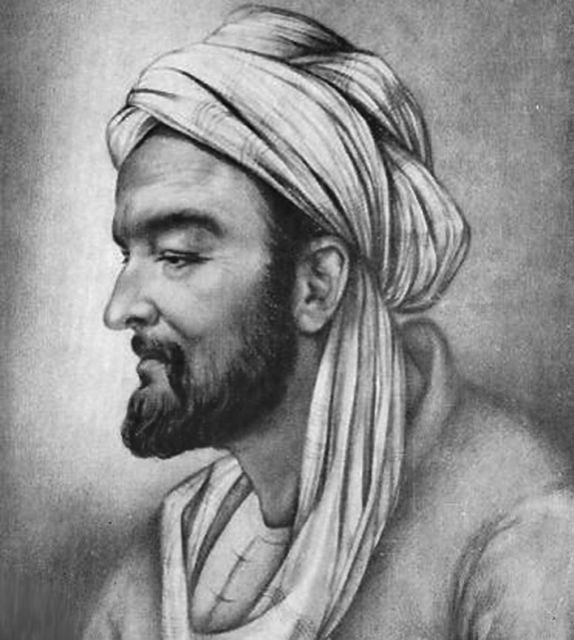
\includegraphics[width=5cm]{abu_ali.jpg}
  \caption*{«Коль смолоду избрал к заветной правде путь, \\
 С невеждами не спорь, советы их забудь». }
 \end{center}
\end{figure}


Каждый Мудрец может постигнуть Истину самостоятельно с вероятностью $1/9$ или же от соседа\footnote{Студенты постигают Истину примерно также!}. Независимо от способа постижения Истины, просветлённый Мудрец поделится Истиной с соседом слева с вероятностью $2/9$ и с соседом справа также с вероятностью $2/9$ (независимо от соседа слева).


\begin{enumerate}
\item Какова вероятность того, что Абу Али Хусейн ибн Абдуллах ибн аль-Хасан ибн Али ибн Сина постигнет Истину?
\item Как изменится ответ, если ряд Мудрецов бесконечен в обе стороны?
\end{enumerate}

\end{enumerate}

\end{document}
